\chapter{Documento de Visão}

A finalidade deste documento é coletar, analisar e definir necessidades e recursos de nível superior do Sistema de Comunicação Interveicular para Alertas de Colisões em Rodovias (CIAC). Ele se concentra nos recursos necessários aos envolvidos e aos usuários-alvos e nas razões que levam a essas necessidades. Os detalhes de como o CIAC satisfaz essas necessidades são descritos nas especificações de requisitos.

\begin{itemize}


\item \textbf{Posicionamento}:  No Brasil há um grande número de colisões frontais nas rodovias federais devido a ultrapassagens, assim como pode ser observado nos dados obtidos no site do IPEA \ref{fig:numero_acidentes}.


\begin{figure}[h!]
\centering
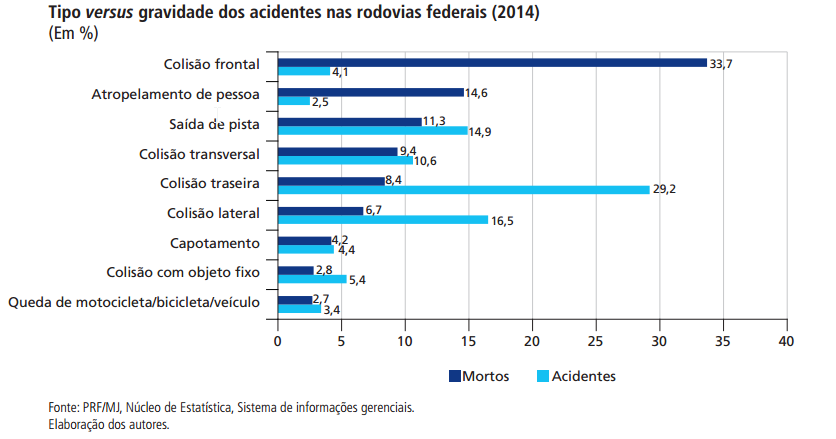
\includegraphics[width=250px, scale=1]{figuras/numero_acidentes}
\caption{Número de acidentes em rodovias}
\label{fig:numero_acidentes}
\end{figure}

Nos últimos dez anos, o Brasil registrou aumento de 50,3\% no número de acidentes em rodovias federais. As mortes cresceram
34,5\% e a quantidade de feridos, 50\%. Mas, nos últimos quatro anos, esses números vêm reduzindo; de 2010 a 2014, as mortes
diminuíram aproximadamente 4,5\%. As colisões frontais e atropelamentos são tipos de acidentes que apresentam baixa
 ocorrência (6,5\% do total em 2014), mas respondem por quase metade (48,3\%) das mortes nas rodovias federais. Os
 automóveis estão envolvidos na maior parte dos acidentes nas rodovias (75,2\%). Justamente a falta de atenção dos
 motoristas que faz com que as colisões frontais, oriundas de ultrapassagens perigosas, representem 34\% das mortes, de
 acordo com a Polícia Rodoviária Federal (PFR) \cite{ipea3}.

 \item \textbf{Oportunidade de Negócio}: O Sistema de Comunicação Interveicular para Alertas de Colisões em Rodovias (CIAC) será projetado para prevenir acidentes de colisões  frontais em rodovias brasileiras, por meio de alertas para o condutor do veículo quando a ultrapassagem não for segura, ou seja, ocasionará batida entre os dois automóveis. Além disso, diminuirá a incerteza do condutor em avaliar se a manobra será realizada com sucesso, com a indicação se o momento é adequado ou não para efetuá-la.

A expectativa é que com a atuação do CIAC, os índices de acidentes em rodovias apresentados acima, sejam reduzidos, além de se esperar um aumento na segurança do condutor e passageiros ao trafegarem pelas rodovias brasileiras.

  \item  \textbf{Descrição do Problema}


\subsection{Descrição do Problema}
\begin{table}[ht]
\caption{Framework do Problema}
\centering
\begin{tabular}{| l |  p{7cm} |}
\hline
O problema da & Acidentes por colisões frontais em rodovias brasileiras  \\
\hline
Afeta & Motoristas de automotores que trafegam pelas rodovias de mão única, Governo do Brasil. \\
\hline
Cujo o impacto é & Número de acidentes nas rodovias, aumento nos gastos com hospitais por parte do Estado brasileiro.\\
\hline
Uma boa solucao seria & Ter um sistema de transmissão de dados de posição dos carros para alertar os motoristas sobre a impossibilidade da ultrapassagem. \\
\hline
\end{tabular}
\end{table}


\item \textbf{Sentença de Posição do Produto}

\begin{table}[h!]
\caption{Sentença de Posição do Produto}
\centering
\begin{tabular}{| p{5cm} |  p{7cm} |}
\hline
Para & Motoristas, Governo do Brasil. \\
\hline
Que & Desejam ter informações sobre a rodovia e carros próximos para poder ultrapassar com segurança. \\
\hline
O Sistema de Comunicação Interveicular para Alertas de Colisões em Rodovias (CIAC) &É um dispositivo que permite o motorista ter ideia dos carros que se encontram perto dele, raio de 4 km, e emite alertas sonoros e visuais caso seja identificado uma ultrapassagem potencialmente perigosa por parte do condutor. \\
\hline
Que & por meio de sistemas como o Transpônder emite e capta informações obtidas através do GPS e outros sistemas embarcados. \\
\hline
Diferente de & Outros dispositivos que não se comunicam com outros veículos na rodovia e os avisa das condições de um conjunto de veículos.  \\
\hline
Nosso Produto & Oferece informações sobre o estado atual do carro para. \\
\hline
\end{tabular}
\end{table}


\item \textbf{Descrição dos Envolvidos e dos Usuários}

\begin{table}[h!]
\caption{Descrição dos Envolvidos e dos Usuários}
\centering
\begin{tabular}{| p{3cm} |  p{5cm} | p{5cm} |}
\hline
Nome & Descrição & Responsabilidades \\
\hline
DetranEstado & Departamento de Trânsito do estado responsável pela rodovia ou determinada região da rodovia. & Responsável por cumprir e fazer cumprir a legislação e normas de trânsito. Segundo lei 9.503 de 23 de setembro de 1997,Art 22. \\
\hline
DNIT & Departamento Nacional de Infraestrutura de Transportes & Implementar a política de infraestrutura do Sistema Federal de Viação, compreendendo sua operação, manutenção, restauração ou reposição, adequação de capacidade e ampliação mediante construção de novas vias e terminais. \\
\hline
\end{tabular}
\end{table}


\item \textbf{Resumo dos Usuários}

\begin{table}[h!]
\caption{Resumo dos Usuários}
\centering
\begin{tabular}{| p{3cm} |  p{5cm} | p{5cm} |}
\hline
Nome & Descrição & Responsabilidades \\
\hline
Motorista & Usuário de veículo automotor presente no Art 96. do Codigo de Trânsito Brasileiro, excluindo os seguintes veículos:

De propulsão humana ou tração animal

Motonetas, motocicletas,ciclomotor, triciclo,quadriciculo. & Através de seu veículo ,integrado com o dispositivo a ser desenvolvido, emitir informações a respeito de sua posição na rodovia e velocidade média.
 \\
\hline
\end{tabular}
\end{table}

\item \textbf{Perspectivas do Produto}
Através do Sistema de Comunicação Interveicular para Alertas de Colisões em Rodovias espera-se que o número de acidentes em rodovias de mão única seja reduzido dando visão para o motorista sobre os veículos nas redondezas. Por meio de informações coletadas através de diferentes dispositivos. Espera-se também uma ligeira redução nos gastos públicos em decorrência dos acidentes e fatalidades como apresentadas na Introdução deste documento.

Software

O software será responsável por fazer a comunicação entre os diversos componentes eletrônicos e garantir que as informações sejam processadas corretamente, além de exibir informações como velocidade, veículos próximos, distâncias para o usuário, com a informação da viabilidade da ultrapassagem, ou alerta do perigo da manobra a ser realizada. Dessa forma, o software deverá ser em um hardware capaz de atender a estas necessidades de processamento.


Energia

As baterias automotivas são utilizadas para manter o sistema em funcionamento, são baterias recarregáveis. Elas armazenam energia sob a forma química para ser transformada em elétrica e utilizada pelo veículo e o CIAC. Estas necessitam suprir a necessidade energética de ambos os sistemas, além de se manter carregada.

Eletrônica

A câmera colhe informações do tráfego dos veículos e a posição do veículo na pista, com objetivo de diminuir os erros de dados do sistema.

Necessidade de um sensor que possibilite  identificar quando o motorista apresenta intenção de ultrapassar, foi escolhe-se um sensor de rotação que identifique a posição angular da direção do veiculo, onde ao girar o volante no sentido da ultrapassagem, deve calcular a angulação de giro para ser processado pelo processador. as ações do sistema.

Para auxiliar o sistema será usado um laser, o funcionamento desses sistemas, consiste, basicamente em, emitir um feixe de luz, que chega ao receptor após algum tempo, com base no tempo que demora para o feixe percorrer o espaço até seu obstáculo e em seguida até seu receptor, e na velocidade da luz, é possível calcular a distância da fonte ao obstáculo.

O Sistema de Posicionamento Global, GPS, será utilizado para mostrar a localização dos veículos no mapa, assim como suas respectivas velocidades e distâncias entre os carros, com dependência de um sinal de triangulação com os satélites geoespaciais.

Para a transmissão de informações entre os veículos, tais como velocidade de posição geográfica, necessita-se de um transponder e dessa forma consegue-se que esses dados, necessários aos cálculos base do sistema sejam obtidos com maior segurança visto que ele utiliza de ondas eletromagnéticas para a transmissão das informações,

\end{itemize}
